\documentclass[12pt]{article}
\usepackage[utf8]{inputenc}
\usepackage{amsmath}
\usepackage{amssymb}
\usepackage{graphicx}
\usepackage{comment}

\graphicspath{ {./plots/} }

\newcommand{\rectres}[1]{
\begin{center}
\begin{tabular}{ |c| }
\hline
\\
 #1\\
 \\
\hline
\end{tabular}
\end{center}
}

\newcommand{\qed}{\hfill$\blacksquare$}

\title{Introduction to Numerical Optimization\\Assignment 4}
%\author{Yair Nahum 034462796\\and\\blabla 11111111 }
\author{}

\begin{document}

\maketitle

%\tableofcontents{}

\section{Augmented Lagrangian method for Constrained Optimization}

\subsection{Graph}

We need to consider the following quadratic programming problem:
\begin{gather*}
    \min_{x_1,x_2}  2(x_1-5)^2 + (x_2-1)^2 \\
    \text{s.t \quad}\begin{array}{lr}
        x_2 \leq 1 - 0.5x_1 \\
        x_2 \geq x_1 \\
        x_2 \geq -x_1
    \end{array}
\end{gather*}
Which can be written as:
\begin{gather*}
    \min_{x_1,x_2}  2x^2_1-20x_1+100  + x^2_2-2x_2+1 \\
    \text{s.t \quad}\begin{array}{lr}
        0.5x_1 + x_2 -1 \leq 0  \\
        x_1- x_2 \leq 0 \\
        -x_1- x_2 \leq 0
    \end{array}
\end{gather*}
Or with matrices as:
\begin{gather*}
    \min_{x}  x^TAx + b^Tx + c \\
    \text{s.t \quad}\begin{array}{lr}
        Bx + d  \leq 0
    \end{array}
\end{gather*}
when:

\begin{itemize}
  \item $A \in \mathbb{R}^{2 \times 2}, A = \begin{bmatrix}
               2 & 0 \\
               0 & 1 \\
  \end{bmatrix}, x,b \in \mathbb{R}^{2}, b = \begin{bmatrix}   -20 \\ -2\\ \end{bmatrix}, c \in \mathbb{R}, c= 101$ 
  \item $B \in \mathbb{R}^{3 \times 2}, B = \begin{bmatrix}
               0.5 & 1 \\
               1 & -1 \\
               -1 & -1 \\
  \end{bmatrix}, d \in \mathbb{R}^{3}, d = \begin{bmatrix}   -1 \\ 0\\ 0\\\end{bmatrix}$
\end{itemize}

We plot the objective function contours (ellipses as we have different eigen values in our A matrix) and the constraints:\\
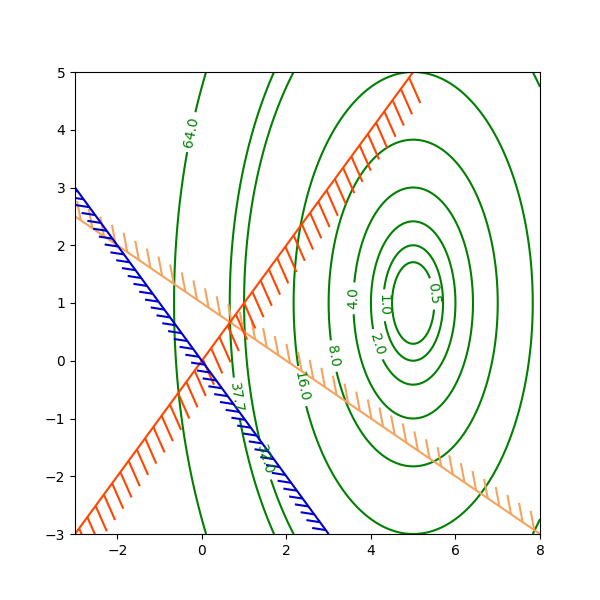
\includegraphics[scale=0.5]{hw4/plots/plot_1.png}\\
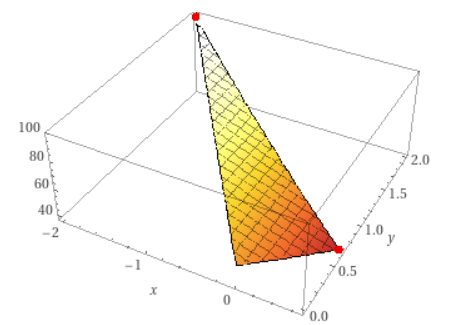
\includegraphics[scale=0.5]{hw4/plots/plot_2.png}\\
From plot, we can see the active constraints are the red and yellow together (the intersection point) and the blue ($-x_1- x_2 \leq 0$) is none active.

\subsection{Optimal Solution}

The intersection of the 2 active constraints is both are satisfied:
$$x_1=x_2, 0.5x_1+x_2=1 \Rightarrow x=(x_1,x_2)=(\frac{2}{3},\frac{2}{3}), f^*(x) = 37\frac{2}{3}$$

\subsection{Optimal Solution}



















\begin{comment}

\section{Constrained Optimization and Duality}

\subsection{Question 1}
We need to solve the following 
\begin{equation}
\label{eq:min1}
\begin{split}
    \min _x x^T M x + c^T x \\
    \text{s.t. } Ax = b
\end{split}
\end{equation}
Given:
\begin{itemize}
  \item $M \in \mathbb{R}^{n\times n},M \succ 0$
  \item $A \in \mathbb{R}^{m\times n}$
  \item $x,c \in \mathbb{R}^{n}$
  \item $b \in \mathbb{R}^{m}$
  \item Assuming $M$ and $AM^{-1}A^T$ are invertible.
\end{itemize}
M is P.D $\Rightarrow$ it is Hermitian ($M=M^*$), and since $M \in \mathbb{R}^{n\times n}$ it is symmetric($M=M^T$).\\
We require the KKT conditions (necessary conditions for $x^*$ to be optimal).\\
These conditions hold as this is a convex problem with only linear constraints.
The Lagrangian is:
$$L(x,\mu)=x^T M x + c^T x + \mu^T(Ax-b)$$
The first KKT condition $\nabla_x L(x,\mu)=0$:
$$\nabla_x L(x,\mu)=0 = 2Mx + c + A^T\mu \Rightarrow$$
$$x^* = -\frac{1}{2}M^{-1}(c + A^T\mu^*)$$
The $M$ is invertible since it is P.D.\\
The third KKT condition gives $h_i(x)=Ax-b=0$, if we put the $x^*$ in it we can isolate and get $\mu^*$:\\
$$-\frac{1}{2}AM^{-1}(c + A^T\mu^*) = b \Rightarrow$$
$$b+\frac{1}{2}AM^{-1}c = -\frac{1}{2}AM^{-1}A^T\mu^* \Rightarrow$$
$$\mu^* = -(AM^{-1}A^T)^{-1}(2b+AM^{-1}c)$$
We put back in $x^*$ :\\
$$x^* = -\frac{1}{2}M^{-1}(c + A^T\mu) =-\frac{1}{2}M^{-1}(c + A^T(-(AM^{-1}A^T)^{-1}(2b+AM^{-1}c))) \Rightarrow $$
\rectres{$$x^* =  \frac{1}{2}M^{-1}(A^T(AM^{-1}A^T)^{-1}(2b+AM^{-1}c)-c)$$}
\newpage
\subsection{Question 2}

We need to solve the following 
\begin{equation}
\label{eq:min2}
\begin{split}
    \min _x ||x - c||^2_2 \\
    \text{s.t. } Ax = b
\end{split}
\end{equation}
Given:
\begin{itemize}
  \item $A \in \mathbb{R}^{m\times n}$
  \item $x,c \in \mathbb{R}^{n}$
  \item $b \in \mathbb{R}^{m}$
  \item Assuming $AA^T$ is invertible.
\end{itemize}

We require the KKT conditions (necessary conditions for $x^*$ to be optimal).\\
These conditions hold as this is a convex problem with only linear constraints.
The Lagrangian is:
$$L(x,\mu)=x^Tx -2c^T x + c^Tc + \mu^T(Ax-b)$$
The first KKT condition $\nabla_x L(x,\mu)=0$:
$$\nabla_x L(x,\mu)= 0 = 2x -2c + A^T\mu \Rightarrow$$
$$x^* = (c - \frac{1}{2} A^T\mu^*)$$
The third KKT condition gives $h_i(x)=Ax-b=0$, if we put the $x^*$ in it we can isolate and get $\mu^*$:\\
$$b = A(c - \frac{1}{2} A^T\mu) \Rightarrow$$
$$\mu^* = 2(AA^T)^{-1}(Ac-b)$$
We put back in $x^*$ :\\
$$x^* = c - \frac{1}{2} A^T\mu^* = c - \frac{1}{2} A^T (2(AA^T)^{-1}(Ac-b))  \Rightarrow  $$
\rectres{$$x^* =   c - A^T(AA^T)^{-1}(Ac-b)$$}

\newpage

\subsection{Question 3}

\begin{equation}
\label{eq:min3}
\begin{split}
    \min _x x^T A x + b^T x \\
    \text{s.t. } \\
    1^T_3x = 1\\
    x_3 \leq 1\\
\end{split}
\end{equation}
Given:
\begin{itemize}
  \item $A \in \mathbb{R}^{3 \times 3}$
  \item $x,b,1_3 \in \mathbb{R}^{3}$
  \item $A = \begin{bmatrix}
               1 & 1 & 0 \\
                1 & 2 & 0 \\
                0 & 0 & 0 \\
              \end{bmatrix}$
  \item $b = \begin{bmatrix}  1 \\ -1 \\ 1\\ \end{bmatrix}$
  \item $1_3 = \begin{bmatrix} 1\\  1\\  1\\ \end{bmatrix}$
\end{itemize}

\subsubsection{Is the problem convex?}
Since the constraints functions are linear $g_i(x),h_i(x)$ they are also convex.\\
The target function is convex iff $A\succcurlyeq 0$.
To check this, we can check all the principal minors to be $M_{i,i}\geq 0$ or by finding all eigenvalues to be $\lambda_i \geq 0$. 
\begin{itemize}
  \item There are 7 principal minors for $3\times3$ matrix $m=2^n-1$. The minors are: 1 ,2 ,0, 0, 0 ,1 ,0. so we found that all are greater or equal to 0. Therefore, $A\succcurlyeq 0$.
  \item Finding the eigenvalues by $det(\lambda I - A) = 0 \Rightarrow$:\\
  $$0=\lambda((\lambda-2)(\lambda-1)-1)=\lambda(\lambda^2-3\lambda+1)\Rightarrow$$
  $$\lambda_1=0, \lambda_{2,3}=\frac{3\pm \sqrt{5}}{2} \Rightarrow$$
  All eigenvalues are greater or equal to 0. Therefore, $A\succcurlyeq 0$.
\end{itemize}
Bottom line, the problem is convex as $A$ is positive semi definite. 
\subsubsection{Find and solve the dual problem}
Since the problem is convex and the constraints are linear, the Slater's condition (SC) holds and the strong duality is valid.\\
Let's first define the primal problem.\\
The constraints:\\
$$g_1(x)=\begin{bmatrix}  0 & 0 & 1 \end{bmatrix}^T x - 1\leq 0$$
$$h_1(x)=1^T_3 x - 1 = 0$$
The Lagrangian is as follows:\\
$$L(x,\mu,\lambda)=x^T A x + b^T x + \mu_1 h_1(x) + \lambda_1 g_1(x)$$
The primal problem is therefore:
$$p* = \min _x \max _{\mu,\lambda \geq 0} L(x,\mu,\lambda)$$
The dual function is:
$$\eta(\mu,\lambda) = \min _x L(x,\mu,\lambda) $$
The dual problem is therefore:
$$d* =  \max _{\mu,\lambda \geq 0} \min _x L(x,\mu,\lambda) = \max _{\mu,\lambda \geq 0} \eta(\mu,\lambda)$$
The KKT conditions hold. Let's solve the dual problem.\\
We can find $\eta(\mu,\lambda) = \min _x L(x,\mu,\lambda)$ (the optimal $x^*$ for specific $\mu,\lambda$) by the KKT condition $\nabla_x L(x,\mu,\lambda) = 0$:
$$\nabla_x L(x,\mu,\lambda) = 2Ax + b + \mu_1 1_3 + \lambda_1 \begin{bmatrix}  0 \\ 0 \\ 1 \end{bmatrix} = 0 \Rightarrow$$
$$ 2 \begin{bmatrix} 1 & 1 & 0 \\ 1 & 2 & 0 \\ 0 & 0 & 0 \\ \end{bmatrix} x + 
\begin{bmatrix}  \mu_1 + 1 \\ \mu_1 - 1 \\ \mu_1 + \lambda_1 + 1\\ \end{bmatrix} = 0 \Rightarrow$$
We get 3 equations:\\
\setcounter{equation}{0}
\begin{equation}
2x_1 + 2x_2 +\mu_1 + 1 = 0
\end{equation}
\begin{equation}
2x_1 + 4x_2 +\mu_1 - 1 = 0
\end{equation}
\begin{equation}
\mu_1 + \lambda_1 + 1 = 0
\end{equation}
By subtracting equations (2) - (1) we get $x_2$:
$$2x_2 = 2 \Rightarrow x_2 = 1$$
Therefore, $x_1$:
$$x_1 = -\frac{1}{2}(\mu_1+3)$$
From the third KKT condition (the constraints) we get:
$$1_3^T x = 1 \Rightarrow$$
$$x_3 = -x_1 = \frac{1}{2}(\mu_1+3)$$
So, we got the following expression for $x*$:
$$x^* = \begin{bmatrix}  -\frac{1}{2}(\mu_1+3) \\ 1 \\ \frac{1}{2}(\mu_1+3) \end{bmatrix}$$
Providing the constraint:
$$\mu_1 + \lambda_1 + 1 = 0$$
Setting the $x^*$ in the Lagrangian, we get the dual function:
$$\eta(\mu,\lambda) = \min _x L(x,\mu,\lambda) = L(x^*,\mu,\lambda) = x^{*T} A x^* + b^T x^* + \mu_1 (1_3^T x^* - 1) + \lambda_1 (x^*_3-1)$$
$$x^{*T} A x^* = \begin{bmatrix}  x^*_1 & x^*_2 & x^*_3 \end{bmatrix} 
\begin{bmatrix} 1 & 1 & 0 \\ 1 & 2 & 0 \\ 0 & 0 & 0 \\ \end{bmatrix} 
\begin{bmatrix}  x^*_1 \\ x^*_2 \\ x^*_3 \end{bmatrix} = $$
$$\begin{bmatrix} x^*_1+1  & x^*_1+2 & 0 \end{bmatrix}
\begin{bmatrix}  x^*_1 \\ 1 \\ x^*_3 \end{bmatrix}
 =x^*_1^2 + 2x^*_1 + 2$$
$$ b^T x^* = \begin{bmatrix}  1 & -1 & 1 \end{bmatrix} \begin{bmatrix}  x^*_1 \\ 1 \\ -x^*_1 \end{bmatrix} = -1$$
Combining it together we get the dual function after minimizing by x:
$$\eta(\mu,\lambda) =  L(x^*,\mu,\lambda) = x^*_1^2 + 2x^*_1 + 2 - 1 + \lambda_1 (x^*_3-1) = x^*_1^2 + (2-\lambda_1) x^*_1 + 1 - \lambda_1  =$$
$$\frac{1}{4}(\mu_1 + 3)^2 + (\lambda_1-2) (\frac{1}{2}(\mu_1+3) + 1 - \lambda_1$$

The dual problem is therefore:
\rectres{
$$d^* =  \max _{\mu_1,\lambda_1} [ \frac{1}{4}(\mu_1 + 3)^2 + (\lambda_1-2) (\frac{1}{2}(\mu_1+3) + 1 - \lambda_1 ] \\ \text{s.t. } \mu_1 + \lambda_1 + 1 = 0, \lambda_1 \geq 0$$
}
Solving the dual problem, we use the linear constraint (part of KKT conditions that the constraint holds) $ \lambda_1 = - \mu_1 - 1$ and put it in the target function:
$$\eta(\mu,\lambda) = [ \frac{1}{4}(\mu_1 + 3)^2 + (\lambda_1-2) (\frac{1}{2}(\mu_1+3) + 1 - \lambda_1 ] = [ \frac{1}{4}(\mu_1 + 3)^2 - (\mu_1+3) (\frac{1}{2}(\mu_1+3) + 2 + \mu_1 ] = $$ $$\frac{\mu_1^2+6\mu + 9}{4} - \frac{\mu_1^2+6\mu_1 + 9}{2} + 2 + \mu_1 = - \frac{\mu_1^2+6\mu_1 + 9}{4} + 2 + \mu_1 =  \frac{-\mu_1^2 -6\mu_1 - 9 + 8 + 4\mu_1}{4}=$$
$$\frac{-\mu_1^2 -2\mu_1 - 1}{4}$$
We can see that this is a concave function, therefore it has a maximum.\\
Calculating the derivative and compare to 0 we get:
$$\eta'(\mu_1) = \frac{-\mu_1 -1}{2} = 0 \Rightarrow$$
$$\mu_1^* = -1$$
And by the constraint:
$$\lambda^*_1 = 0$$
Putting it back in $x*$ we get:\\
$$x^* = \begin{bmatrix}  -\frac{1}{2}(\mu_1+3) \\ 1 \\ \frac{1}{2}(\mu_1+3) \end{bmatrix} = \begin{bmatrix}  -1 \\ 1 \\ 1 \end{bmatrix}$$
And the function minimum value:
$$f*=p*=d*=\frac{-\mu_1^2 -2\mu_1 - 1}{4} = 0$$
\rectres{
$$x^* = \begin{bmatrix}  -1 \\ 1 \\ 1 \end{bmatrix}, f* = 0$$
}
\newpage
\subsection{Question 4}
We need to find and write the dual problem of the following linear programming problem:
\setcounter{equation}{0}
\begin{equation}
\label{eq:min4}
\begin{split}
    \min _x c^T x \\
    \text{s.t. }\\
    Ax \leq b\\
    x \geq 0
\end{split}
\end{equation}
Given:
\begin{itemize}
  \item $A \in \mathbb{R}^{m\times n}$
  \item $x,c \in \mathbb{R}^{n}$
  \item $b \in \mathbb{R}^{m}$
\end{itemize}
First we will define the primal problem:
$$p^*=\min_x \max_{\mu,\lambda \geq 0} L(x,y,\lambda)$$
When the Lagrangian is:
$$L(x,y,\lambda) = c^T x + y^T (Ax-b) -\lambda^T x$$
$$\\y,\lambda \in \mathbb{R}^m$$

The problem is convex with linear only constraints, so by Slater's condition we have strong duality.\\
That is:
$$p^*=\min_x \max_{y \geq 0,\lambda \geq 0} L(x,y,\lambda) = \max_{y \geq 0,\lambda \geq 0} \min_x  L(x,y,\lambda) = d^*$$
The dual function $\eta(y,\lambda)$ is:
$$\eta(y,\lambda) = \min_x  L(x,y,\lambda)$$
To find the dual problem, we will compare the $\nabla_x (x,y,\lambda)$ to zero according to KKT conditions:\\
$$\nabla_x (x,y,\lambda) = c + A^Ty - \lambda = 0$$
This means that the dual problem has a constraint:\\
$$c = \lambda-A^Ty $$
From complementary slackness $y^T (Ax-b) -\lambda^T x= 0 \Rightarrow$:
$$(y^T A - \lambda^T)x - y^Tb = 0 \Rightarrow $$
$$-c^Tx - y^Tb = 0 \Rightarrow c^Tx = - y^Tb$$
And therefore the Lagrangian doesn't depend on x:\\
$$L(x,y,\lambda) = - y^Tb$$
(BTW, we can also get the Lagrangian by just setting $c=\lambda -A^Ty$)\\
So, the dual function is:
$$\eta(y,\lambda) = \min_x  L(x,y,\lambda) = \begin{cases}
			- y^Tb, & \text{if } c + A^Ty = \lambda\\
            -\infty, & \text{otherwise}
		 \end{cases}$$
To conclude, the dual problem is:
\rectres{
$$f^* = p^* = d^* = \max_y - y^Tb$$\\
$\text{s.t. } \lambda \geq 0, y \geq 0, c + A^Ty = \lambda$
}

\end{comment}

\end{document}

